\documentclass[journal]{IEEEtran}
\usepackage{amsmath,amsfonts}
\usepackage{algorithmic}
\usepackage{array}
\usepackage[caption=false,font=normalsize,labelfont=sf,textfont=sf]{subfig}
\usepackage{textcomp}
\usepackage{stfloats}
\usepackage{url}
\usepackage{verbatim}
\usepackage{graphicx}
\hyphenation{op-tical net-works semi-conduc-tor IEEE-Xplore}
\def\BibTeX{{\rm B\kern-.05em{\sc i\kern-.025em b}\kern-.08em
    T\kern-.1667em\lower.7ex\hbox{E}\kern-.125emX}}
\usepackage{balance}
\begin{document}
\title{Situation-Aware Integrated Sensing and Communication for 6G Smart Warehouses: A Sionna RT and ns-3 Co-Simulation Framework}
\author{
  \IEEEauthorblockN{Aung Kaung MYAT, Hrishikesh Dutta, Roberto Minerva, Noel Crespi}\\
    \IEEEauthorblockA{\textit{SAMOVAR, Télécom SudParis} \\
    \textit{Institut Polytechnique de Paris}\\
    Palaiseau, France \\
    Email: \{aung-kaung.myat, hrishikesh.dutta, roberto.minerva, noel.crespi\}@telecom-sudparis.eu
  }
}

\markboth{Journal of \LaTeX\ Class Files,~Vol.~18, No.~9, September~2020}%
{Situation-Aware Integrated Sensing and Communication for 6G Smart Warehouses}

\maketitle

\begin{abstract}
Smart warehouses need wireless networks that can support sensors, controllers,
video traffic, and mobile robots while also reacting to changes in the
environment. This paper presents a situation-aware Integrated Sensing and
Communication (ISAC) co-simulation framework that connects Sionna RT ray
tracing with ns-3/5G~LENA networking. The framework uses ray-traced multipath
to detect reflected targets, filters clutter, tracks moving objects, and then
uses the confirmed target positions to form sensing-informed beams.

The framework is evaluated in two stages. First, controlled free-space and
warehouse scenes are used to test the sensing and beamforming pipeline under
clear and cluttered conditions. Second, an end-to-end warehouse Digital Twin is
used to study the same mechanism with mobile robots, package and rack sensors,
cameras, video clients, and mixed application traffic. The controlled results
show that ISAC reduces path loss in both scenes, that a wider beam gives the
best communication behavior, and that tracking is needed to suppress false
detections. Deeper propagation gives a small detection gain, but it can also
increase clutter in the warehouse. In the full warehouse use case, the
$4{\times}4$ gNB array gives the best balance: the $2{\times}2$ array is not
stable enough, while the $8{\times}8$ array increases power consumption without
a proportional performance gain. These results show that practical ISAC
evaluation must consider sensing quality, communication performance, and energy
cost together.
\end{abstract}

\begin{IEEEkeywords}
Integrated sensing and communication (ISAC), 6G, situation awareness, ray
tracing, Sionna RT, ns-3, 5G LENA, adaptive beamforming, multi-target tracking,
Digital Twin, smart warehouse.
\end{IEEEkeywords}


\section{Introduction}
\label{sec:introduction}

The evolution toward 6G networks is driven by the need to support increasingly
complex and dynamic applications, including Digital Twins (DT), autonomous
systems, and intelligent environments. Among these, smart-warehouse systems
represent a particularly challenging use case, where mobile robots, sensing
devices, and control systems must operate reliably under stringent latency,
reliability, and throughput requirements. In such environments, the wireless
network is no longer a passive communication medium: it becomes an active
component of the system that must adapt continuously to changes in user
position, mobility patterns, and environmental conditions. This motivates the
concept of \emph{situation awareness}, in which the communication system
leverages contextual information to optimise its behaviour proactively rather
than reactively~\cite{ref:positioning_6g}.

Situation awareness, in the context of wireless access networks, refers to the
ability of the network---particularly the antenna system and its associated
control logic---to perceive and exploit contextual information such as user
equipment (UE) location, mobility trajectories, surrounding geometry, and
potential obstacles. Instead of relying on periodic beam training or
threshold-based handovers, a situation-aware system anticipates future channel
conditions and adapts accordingly. In a smart-warehouse setting, this
includes predicting robot movement along planned paths, identifying potential
blockages from racks or moving objects, and adjusting beamforming strategies
to maintain reliable links. Such proactive adaptation has been shown to
improve key performance indicators (KPIs) including latency, throughput,
reliability, and energy efficiency, particularly in higher-frequency bands
where propagation is highly sensitive to environmental
dynamics~\cite{ref:multimodal_bf,ref:predictive_handover}.

Enabling situation awareness, however, requires the network to have access to
accurate and timely environmental information. Conventional radio measurements
such as RSRP or SINR provide limited insight into the physical environment and
often arrive too late to support proactive adaptation. To overcome this
limitation, the antenna system must be endowed with \emph{sensing
capabilities}, allowing it to observe the surrounding environment and infer
the position and motion of objects directly. This convergence of sensing and
communication functionalities is a fundamental requirement for next-generation
networks and forms the basis of the Integrated Sensing and Communication
(ISAC) paradigm. ISAC integrates radar-like sensing into the communication
infrastructure so that the same hardware, waveform, and spectrum are jointly
used for data transmission and environmental sensing. In a smart warehouse,
ISAC enables a base station to detect and track mobile robots and other
dynamic objects from reflected signals, transforming the communication system
into a distributed sensing platform without dedicated sensing infrastructure.

A key challenge in studying ISAC systems lies in faithfully modelling the
interaction between electromagnetic waves and complex environments.
Conventional system-level simulators rely on stochastic channel models that do
not capture site-specific reflections, diffractions, and blockages. To address
this, ray-tracing techniques are employed as a high-fidelity modelling
approach: by leveraging detailed scene geometry and material properties, ray
tracing provides per-path delays, angles of arrival/departure, and complex
gains, which are essential both for accurate communication modelling and for
the radar-like reasoning that underpins
sensing~\cite{ref:sionna_rt,ref:ns3sionna}.

Building on this foundation, this paper presents an ISAC framework that pairs
NVIDIA Sionna RT with ns-3/5G~LENA into a single co-simulation pipeline, and
evaluates it both in controlled scenes and in an end-to-end smart-warehouse
Digital Twin. The contributions of the paper are as follows:
\begin{itemize}
  \item It describes the integration of ns-3/5G~LENA with Sionna RT through a
        ZeroMQ-based propagation/sensing bridge, with a clean role boundary
        between the two simulators (Section~\ref{sec:methodology}).
  \item It presents a four-module ISAC architecture comprising a
        radar-inspired sensing module (Equivalent Reflection Point (ERP)
        computation, $Z$-gating, Moving-Target Indication (MTI), and DBSCAN
        clustering), a Kalman--Hungarian multi-target tracking module, a
        sensing-informed multi-lobe adaptive beamforming module, and a
        communication module that exports per-path channel state back to
        ns-3 (Section~\ref{sec:methodology}).
  \item It validates the framework through a two-stage evaluation: a
        controlled scene-level study across free-space, warehouse, and
        urban-micro street-canyon scenes with six ablation variants, and an
        application-oriented warehouse Digital Twin study under three gNB
        array sizes (Section~\ref{sec:results}).
  \item It identifies the operating regimes in which the proposed framework
        is beneficial, including the $4{\times}4$ gNB configuration as the
        balanced operating point in the smart-warehouse scenario, and
        discusses the remaining limitations and future research directions
        (Sections~\ref{sec:results}--\ref{sec:conclusion}).
\end{itemize}

The remainder of this paper is organised as follows.
Section~\ref{sec:methodology} describes the simulation flow, ISAC
architecture, and the algorithms used in each module.
Section~\ref{sec:results} presents the controlled-validation and
warehouse-use-case results together with a discussion of their implications.
Section~\ref{sec:conclusion} concludes the paper and outlines future work.


\section{Background and Related Work}
\label{sec:literature}

This section first summarises the gains that situation awareness can bring to
next-generation access networks, and then discusses the simulation tooling
that is required to study these gains in a site-specific manner. The latter
discussion directly motivates the choice of ns-3/5G~LENA combined with Sionna
RT adopted in this paper.

\subsection{Benefits of Situation Awareness}

Situation awareness refers to the capability of antenna systems to adapt their
configuration based on contextual information such as UE position, mobility,
environment geometry, obstacles, and temporal channel variation. Recent
studies show that incorporating such awareness leads to substantial gains in
performance, reliability, and efficiency, which can be grouped into four
families.

\subsubsection{Beamforming and Beam Management}
Surveys of AI-enabled multimodal beamforming indicate that combining non-RF
sensors (e.g., LiDAR, radar, GPS) with RF data improves directional accuracy
and reduces the overhead of beam sweeping and alignment, particularly in
mmWave bands where misalignment and rapid channel variation degrade
performance~\cite{ref:multimodal_bf}. Positioning-aided beamforming for mmWave
communications has specifically shown how location information can relax the
complexity of beam training and narrow the search space for optimal beams.

\subsubsection{Mobility and Handover Management}
Context-aware and predictive handover schemes that exploit UE speed,
direction, hysteresis, trajectory history, and signal-quality metrics reduce
handover failures, ping-pong effects, and latency. Memory-full context-aware
predictive mobility management in dual-connectivity 5G networks uses past UE
trajectory and signal measurements to anticipate handover events and reduce
signalling overhead~\cite{ref:predictive_handover}. Surveys on AI-aided
mobility and handover management confirm that machine-learning-based schemes
can sustain seamless connectivity even in ultra-dense deployments and
high-mobility regimes.

\subsubsection{Reliability and Link Stability}
Awareness of obstacles and environmental geometry enables dynamic beam
switching or alternate-path selection, mitigating the impact of blockages
especially in higher-frequency bands. Future networks are expected to rely
heavily on integrated sensing (and positioning) capabilities to improve link
robustness under dynamic conditions~\cite{ref:positioning_6g}.

\subsubsection{Resource Efficiency and Latency Reduction}
Predictive mobility and proactive beam adjustment avoid unnecessary sweeping,
measurement reporting, and control overhead. Deep-learning-based predictive
handover algorithms have been shown to reduce interruption time and improve
resource utilisation; in mobile edge-computing systems, joint optimisation of
connectivity and computation likewise benefits from context-aware decision
rules~\cite{ref:predictive_handover}.

While the literature confirms substantial improvement potential, it also
emphasises trade-offs: acquiring accurate context (position, environment
mapping) has its own overhead, prediction errors can degrade rather than
improve performance, and privacy and hardware constraints must be addressed.

\subsection{Simulation Tooling for ISAC}

Studying situation-aware ISAC requires a simulation environment that captures
both end-to-end networking behaviour and site-specific propagation. Two
simulator families are commonly used as starting points.

\textbf{Simu5G on OMNeT++.} Simu5G provides end-to-end simulation of 5G NR
spanning application, transport, and network layers, with support for MEC,
C-V2X, and dual connectivity. However, its PHY relies on stochastic 3GPP
abstractions, so it lacks site-specific 3D channel modelling and flexible
MIMO configurations. Most critically for ISAC, the OMNeT++ architecture makes
integrating GPU-accelerated ray tracers such as Sionna RT onerous: the
co-simulation bridge requires heavy glue code, Simu5G exposes only
omnidirectional antennas, and the rich channel outputs computed in Sionna
(per-path gains, delays, AoA/AoD) cannot be propagated cleanly to the upper
layers.

\textbf{5G LENA on ns-3.} 5G LENA implements PHY/MAC system-level behaviour
aligned with 3GPP standards and supports full-stack studies, from packet
capture and IP transport up to RAN-layer scheduling and application
flows~\cite{ref:5glena}. By default it uses simplified stochastic channel
models (e.g., 3GPP TR~38.901~\cite{ref:tr38901}) for path loss, fading, and
beamforming, and therefore lacks deterministic 3D geometry awareness. However,
recent work on Ns3Sionna~\cite{ref:ns3sionna} shows that Sionna RT's
GPU-accelerated ray tracing can be integrated directly into ns-3, yielding
high-fidelity site-specific channels within the existing ns-3 stack; the
published Wi-Fi integration serves as a proof of concept and a solid
technical foundation to extend the same approach to 5G LENA. In this
ns-3/LENA path, integration is cleaner and more expressive: both sides expose
MIMO/beamforming configuration, the per-path channel state computed in Sionna
(complex gains, delays, Doppler, AoA/AoD) can be passed through intact, and
the resulting scheduling, link adaptation, and application-layer metrics
faithfully reflect the underlying geometry-driven radio conditions.

For these reasons, the framework presented in this paper pairs 5G LENA with
Sionna~RT~\cite{ref:sionna_rt} and gives each tool a clear role: Sionna
handles the physical and link layers (ray tracing, MIMO arrays/beamforming,
per-path/beam loss and delay), while 5G LENA consumes these geometry-aware
results to drive the upper layers (RLC/PDCP/IP/applications), so that
buffering, congestion control, and application QoE evolve in response to the
same radio conditions produced by Sionna. This division of labour is detailed
in Section~\ref{sec:methodology}.


\section{Framework and Methodology}
\label{sec:methodology}

This section describes the proposed situation-aware ISAC framework. We first
present the smart-warehouse use case that motivates the design, then the
co-simulation architecture and flow, and finally the four functional modules
of the ISAC pipeline together with their underlying algorithms.

\subsection{Smart-Warehouse Use Case}
\label{subsec:warehouse}

The chosen reference scenario is a logistics floor served by a single gNB and
populated by heterogeneous wireless devices: stationary robotic arms along an
intake conveyor, autonomous mobile robots that ferry parcels to and from
storage racks, fixed cameras, environmental sensors (temperature, humidity),
package and rack sensors, and PCs in a control room running monitoring
applications (Fig.~\ref{fig:warehouse_layout}). The floor exhibits three RF
regions---a clear line-of-sight zone, a partially obstructed zone with rack
edges that intermittently shadow links, and a fully obstructed zone (control
room) separated by walls and dense shelving---which exercise the full range
of LOS/NLOS, diffraction, and blockage conditions.

\begin{figure}[t]
  \centering
  % TODO: extract figure from L4.5 PDF (Figure 3 / overview layout)
  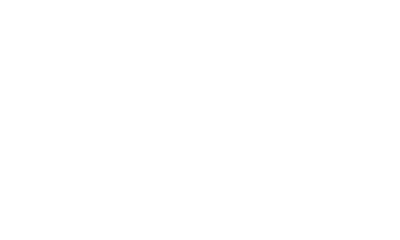
\includegraphics[width=\columnwidth]{images/warehouse_layout.png}
  \caption{Smart-warehouse Digital Twin: a single gNB serves stationary
  robots, autonomous mobile robots, sensors, and fixed cameras across three
  RF regions.}
  \label{fig:warehouse_layout}
\end{figure}

This geometry exercises three progressively more demanding scenarios: a
stationary baseline, predefined mobile paths through mixed-obstruction zones,
and dynamic beamforming with position feedback. The scenario also represents
the broader class of situation-aware use cases identified in our prior work
(smart home, smart warehouse, vehicular networks): all three share the need
for proactive beam steering, predictive handover, and blockage-aware
scheduling. The smart-warehouse case is selected here because it cleanly
combines device heterogeneity, mobility-driven channel variation, and a
controlled indoor geometry suitable for ray-traced sensing.

\subsection{Co-Simulation Architecture}
\label{subsec:architecture}

The end-to-end architecture is shown conceptually in
Fig.~\ref{fig:component_arch}. A remote host runs the application over
TCP/UDP/IP and attaches to the EPC via the PGW/SGW node (\texttt{EpcPgwSgwApp}
over GTP/UDP/IP). On the RAN side, the gNB executes \texttt{EpcEnbApp} and
the LENA NR stack: packets from the core arrive in GTP/UDP/IP, are scheduled
by the NR MAC/PHY, and are forwarded to the gNB's
\texttt{NrGnbNetDevice} for transmission over the air. The UE mirrors this
stack (application $\to$ TCP/UDP $\to$ IP $\to$ \texttt{NrUeNetDevice}), so
end-to-end KPIs (throughput, latency, jitter, loss) are measured natively
within ns-3.

\begin{figure}[t]
  \centering
  % TODO: extract figure from L4.5 PDF (Figure 1, Component Architecture)
  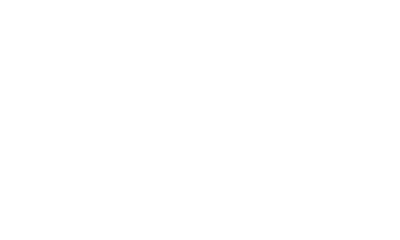
\includegraphics[width=\columnwidth]{images/component_arch.png}
  \caption{End-to-end co-simulation architecture. Sionna RT supplies
  geometry-aware physical-layer realism; ns-3/5G LENA consumes it to drive
  the protocol stack and applications.}
  \label{fig:component_arch}
\end{figure}

Radio propagation is outsourced to a dedicated Sionna ``channel server''
co-located with the RAN. Given the true 3D scene and configured MIMO arrays,
Sionna computes time-varying path sets (per-path gains, delays, Doppler,
AoA/AoD) and returns effective propagation loss and delay---and, when needed,
per-RB SINR estimates---through a ZeroMQ-based adapter. The gNB therefore
performs link adaptation and scheduling against geometry-aware channels that
reflect LOS/NLOS transitions, diffraction, blockage, and beamforming, while
the upper layers react naturally to the resulting radio dynamics.

\subsection{Simulation Flow}
\label{subsec:flow}

In ns-3 we first define the gNB and UE nodes, attach mobility models and
antenna/array configurations, and select the application mix (e.g.,
constant-bit-rate, VoIP, video streaming). The initial positions, MIMO
settings, and application parameters are sent to the Sionna server. Sionna
has already created the 3D scene and an occupancy map, and waits for
requests; upon receiving ns-3's parameters, it initialises the ray-tracing
environment, sets Tx/Rx poses and MIMO patterns, and enters a request/response
loop. Whenever ns-3 asks for channel state, Sionna updates node poses,
estimates paths via ray tracing, optionally adapts the transmit radiation
pattern to the current UE positions, and returns time-aligned propagation
loss and delay reflecting LOS/NLOS transitions, multipath, diffraction, and
blockage. ns-3 ingests these values at the PHY/MAC, performs link adaptation
and scheduling, and the upper layers evolve naturally over those channels.

\subsection{Scene and Mobility Modelling}
\label{subsec:scene}

The 3D scene is loaded from a Blender-exported Mitsuba XML file and
instantiated three times in Sionna RT,
\(\mathcal{S} = \{\mathcal{S}_{\mathrm{sense}},\; \mathcal{S}_{\mathrm{comm}},\;
\mathcal{S}_{\mathrm{bf}}\}\). The three scenes share geometry but differ in
runtime use: $\mathcal{S}_{\mathrm{sense}}$ uses a co-located transmit and
receive array as a monostatic radar; $\mathcal{S}_{\mathrm{comm}}$ uses the
baseline transmitter to compute per-link channel state between the gNB and
UEs; and $\mathcal{S}_{\mathrm{bf}}$ uses a custom multi-lobe radiation
pattern computed from the sensing output. Maintaining three scene instances
avoids repeatedly mutating a single Sionna object between modes.

Mobility is handled by a headless PyBullet backend. Static geometry is loaded
as a mesh, while dynamic objects are loaded as box collision bodies derived
from the bounding box of each mesh. For an object whose mesh occupies
$\mathbf{v}_{\min}=[x_{\min},y_{\min},z_{\min}]^{\!\top}$ and
$\mathbf{v}_{\max}=[x_{\max},y_{\max},z_{\max}]^{\!\top}$, the half-extents
used for collision modelling are
$\mathbf{h} = \tfrac{1}{2}(\mathbf{v}_{\max}-\mathbf{v}_{\min})$. Because
PyBullet operates on the geometric centre while users specify positions at
the base, the centre position is recovered as
\(\mathbf{p}_{\mathrm{centre}} = \mathbf{p}_{\mathrm{bottom}} + [0,0,h_z]^{\!\top}.\)

Path planning uses the A$^{\star}$ algorithm on a 2D grid of resolution $g$.
Each cell $n$ is scored by $f(n)=g(n)+h(n)$, with $g(n)$ the cost-so-far
(straight moves cost $g$, diagonals cost $g\sqrt{2}$) and
$h(n)=\sqrt{(x_n-x_d)^2+(y_n-y_d)^2}$ the Euclidean heuristic to the
destination. Candidate paths are validated against static and dynamic
collisions before commitment. Once accepted, a path is stored as an ordered
list of waypoints $\{w_0,\ldots,w_K\}$, and at simulation time $t \ge t_0$
the agent's traversed length is $s(t)=v\,(t-t_0)$. Defining
$D_0=0$ and $D_k=\sum_{i=1}^{k}\|w_i-w_{i-1}\|_2$, the instantaneous position
on segment $[w_k,w_{k+1}]$ when $D_k\le s(t)\le D_{k+1}$ is obtained by
linear interpolation,
\begin{equation}
  \mathbf{p}(t) = w_k + \alpha\,(w_{k+1}-w_k),
  \qquad
  \alpha = \frac{s(t)-D_k}{D_{k+1}-D_k}.
\end{equation}

\subsection{ISAC Pipeline Overview}
\label{subsec:isac_pipeline}

The ISAC pipeline (Fig.~\ref{fig:isac_arch}) consists of four modules
executed in sequence at every sensing tick: a sensing module that converts
raw ray-tracing output into 3D detections, a multi-target tracking module
that stabilises detections into trajectories, an adaptive beamforming module
that synthesises a custom transmit pattern from the confirmed tracks, and a
communication module that re-runs ray tracing under the new pattern to
produce the per-link channel state delivered to ns-3.

\begin{figure}[t]
  \centering
  % TODO: extract figure from L4.7 PDF (Figure 1, ISAC overview)
  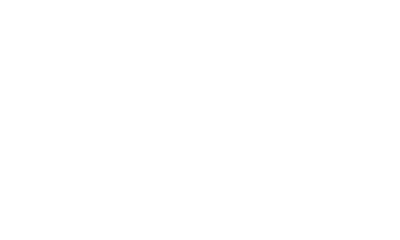
\includegraphics[width=\columnwidth]{images/isac_arch.png}
  \caption{ISAC pipeline: sensing, multi-target tracking, adaptive
  beamforming, and communication.}
  \label{fig:isac_arch}
\end{figure}

\subsection{Ray-Tracing-Based Sensing Module}
\label{subsec:sensing}

The sensing module transforms the ray-traced multipath output into discrete
3D object candidates, following a radar-like reasoning.

\paragraph{Pre-processing.}
For each path $\ell$, the average path power is computed from the complex
coefficients,
\(\overline{P_\ell} = \tfrac{1}{|I|}\sum_{i\in I}|a_{\ell,i}|^2\),
together with the average delay
$\overline{\tau_\ell}=\tfrac{1}{|I|}\sum_{i\in I}|\tau_{\ell,i}|$ and the
average angles $\overline{\theta_\ell}$ and $\overline{\phi_\ell}$. Paths
with $\overline{\tau_\ell}\le 10^{-9}$~s are dropped. The remaining delays
are converted to range, $L_\ell = c\,\overline{\tau_\ell}$.
A distance-adaptive power threshold avoids over-suppressing distant returns,
\begin{equation}
  s_\ell = \max\!\left(\frac{L_\ell}{10},1\right)^{\!1.1},
  \qquad
  P_{\mathrm{th},\ell} = \frac{P_{\min}}{s_\ell},
\end{equation}
and only paths with $\overline{P_\ell}>P_{\mathrm{th},\ell}$ are retained.
Finally, each surviving angle pair is converted to a 3D unit direction,
$\mathbf{d}_\ell=[\sin\theta_\ell\cos\phi_\ell,\sin\theta_\ell\sin\phi_\ell,
\cos\theta_\ell]^{\!\top}$.

\paragraph{Equivalent Reflection Point (ERP).}
Each surviving path is mapped to a single 3D point,
\begin{equation}
  \mathbf{p}_\ell^{\mathrm{ERP}}
  = \mathbf{p}_{\mathrm{gNB}}
  + \!\left(\frac{L_\ell}{2} + \delta\right)\mathbf{d}_\ell,
  \label{eq:erp}
\end{equation}
where $\mathbf{p}_{\mathrm{gNB}}$ is the gNB location, $L_\ell/2$ accounts
for the round-trip in the monostatic case, and $\delta$ is a small
calibration offset that mitigates the bias introduced when reflection occurs
on a surface rather than at the object's centre.

\paragraph{Vertical ($Z$) gating.}
Floor and ceiling reflections produce ghost ERPs that lie outside the height
range of physical targets. A simple gate
\(z_{\min}\le z_\ell^{\mathrm{ERP}}\le z_{\max}\),
calibrated from the target mesh, removes them.

\paragraph{Moving-Target-Indication (MTI) filter.}
The first frame is stored as a static background point cloud
$\mathcal{B}=\{\mathbf{b}_1,\ldots,\mathbf{b}_M\}$. For a new ERP
$\mathbf{p}$, the nearest-background distance is
$d_{\mathcal{B}}(\mathbf{p})=\min_{\mathbf{b}\in\mathcal{B}}\|\mathbf{p}-\mathbf{b}\|_2$,
and only points satisfying $d_{\mathcal{B}}(\mathbf{p})>d_{\mathrm{MTI}}$
are kept. The nearest-neighbour search is implemented with a $k$-d tree.

\paragraph{DBSCAN clustering.}
A real object generates several nearby ERPs, so the surviving cloud is
clustered with DBSCAN~\cite{ref:dbscan}, which does not require the number of
objects in advance, ignores isolated noise, and works well on locally dense
point clouds. For each cluster $\mathcal{C}_k$, the strongest point is taken
as the representative position, $\mathbf{z}_k=\mathbf{p}_{n^\ast}$ with
$n^\ast=\arg\max_{n\in\mathcal{C}_k}\overline{P_n}$, and the cluster power
is $P_k=\sum_{n\in\mathcal{C}_k}\overline{P_n}$. Candidates are sorted by
$P_k$ and pruned: if $\|\mathbf{z}_i-\mathbf{z}_j\|_2 < d_{\mathrm{sep}}$,
the weaker is dropped, so the same physical object is not reported twice.
At most $N_{\max}$ candidates are emitted, each as a tuple
$\mathcal{D}_k=(k,\mathbf{z}_k,P_k)$.

\subsection{Multi-Target Tracking Module}
\label{subsec:tracking}

Raw detections are noisy and intermittent, so they are stabilised by a
constant-velocity Kalman filter with global Hungarian data
association~\cite{ref:hungarian}.

Each target is described by a six-dimensional state
$\mathbf{x}_t = [x_t,y_t,z_t,v_{x,t},v_{y,t},v_{z,t}]^{\!\top}$ that follows
$\mathbf{x}_{t|t-1} = F\mathbf{x}_{t-1|t-1} + \mathbf{w}_t$ with the
constant-velocity transition matrix
\begin{equation}
  F =
  \begin{bmatrix}
    1 & 0 & 0 & \Delta t & 0 & 0 \\
    0 & 1 & 0 & 0 & \Delta t & 0 \\
    0 & 0 & 1 & 0 & 0 & \Delta t \\
    0 & 0 & 0 & 1 & 0 & 0 \\
    0 & 0 & 0 & 0 & 1 & 0 \\
    0 & 0 & 0 & 0 & 0 & 1
  \end{bmatrix},
\end{equation}
and a position-only measurement model $\mathbf{z}_t = H\mathbf{x}_t +
\mathbf{n}_t$ with $H=[I_3\;\;\mathbf{0}_{3\times 3}]$. New tracks are
initialised at the detected position with zero velocity. The filter uses
$P_0=5\,I_6$, $Q=0.1\,I_6$, and $R=1.0\,I_3$, encoding moderate uncertainty
in the initial state, limited deviation from constant velocity, and
non-negligible sensing noise. The default sampling interval is
$\Delta t = 1.0$.

At each frame, all active tracks are propagated by
$\hat{\mathbf{x}}_{t|t-1}=F\hat{\mathbf{x}}_{t-1|t-1}$ and
$P_{t|t-1}=FP_{t-1|t-1}F^{\!\top}+Q$. The current detection set is
de-duplicated by removing any detection within $d_{\mathrm{birth}}$ of a
stronger one. A cost matrix $C\in\mathbb{R}^{N_T\times N_D}$ is then built,
with entries $c_{ij}=\|\hat{\mathbf{p}}_{t|t-1}^{(i)}-\mathbf{z}_{t,j}\|_2$;
entries above the gating threshold $c_{\max}$ are replaced by a large
penalty (1000). The optimal global assignment is obtained by solving
\(\pi^\star = \arg\min_{\pi}\sum_{(i,j)\in\pi}c_{ij}\)
with the Hungarian algorithm. For each accepted pair, a standard Kalman
update is performed,
\begin{align}
  \mathbf{y}_t &= \mathbf{z}_{t,j}-H\hat{\mathbf{x}}_{t|t-1}, \\
  S_t &= HP_{t|t-1}H^{\!\top}+R, \\
  K_t &= P_{t|t-1}H^{\!\top}S_t^{-1}, \\
  \hat{\mathbf{x}}_{t|t} &= \hat{\mathbf{x}}_{t|t-1}+K_t\mathbf{y}_t, \\
  P_{t|t} &= (I-K_tH)P_{t|t-1}.
\end{align}

Unmatched tracks have their missed-frame counter incremented, so short-term
sensing failures (occlusion, weak returns, detector dropout) are tolerated
without immediate deletion. A track is deleted when $m_i\ge M_{\max}$, and a
detection only spawns a new track when its distance to every existing track
exceeds $d_{\mathrm{birth}}$. A track is exported only after it has reached a
minimum age $A_{\min}$ and accumulated displacement
$\|\hat{\mathbf{p}}_i-\mathbf{p}_{\mathrm{start},i}\|_2 > d_{\min}$,
suppressing short-lived false tracks and clutter.

\subsection{Sensing-Informed Adaptive Beamforming}
\label{subsec:beamforming}

Once one or more tracks are confirmed, their estimated positions become
steering points for the communication transmission. For each tracked target
at $\mathbf{p}_m$, the steering vector relative to the gNB is
$\mathbf{u}_m = \mathbf{p}_m-\mathbf{p}_{\mathrm{gNB}}$, with spherical
angles
\(\theta_m = \arccos\!\big(u_{m,z}/\|\mathbf{u}_m\|_2\big)\),
$\phi_m = \mathrm{atan2}(u_{m,y},u_{m,x})$.

Rather than computing a digital precoder, the framework synthesises a custom
antenna element pattern with one Gaussian lobe per tracked target. Let
$\hat{\mathbf{r}}(\theta,\phi)$ denote the unit direction toward the
observation angle and $\hat{\mathbf{r}}(\theta_m,\phi_m)$ the steering
direction toward target $m$. The angular mismatch is
$\psi_m(\theta,\phi)=\arccos\!\big(\hat{\mathbf{r}}(\theta,\phi)^{\!\top}
\hat{\mathbf{r}}(\theta_m,\phi_m)\big)$. With beamwidth parameter
$\sigma=\mathrm{deg2rad}(W)$, the multi-lobe gain is
\begin{equation}
  G(\theta,\phi)
  = \sum_{m=1}^{M}\exp\!\left(-\frac{\psi_m(\theta,\phi)^2}{2\sigma^2}\right).
  \label{eq:multi_lobe}
\end{equation}
An array-level gain compensation $\gamma=200$ is applied and the pattern is
converted to a vertically polarised field amplitude,
\begin{equation}
  A_\theta(\theta,\phi) = \sqrt{\max(G(\theta,\phi),10^{-6})}\,\gamma,
  \quad A_\phi(\theta,\phi) = 0.
\end{equation}
The pattern is regenerated only when the rounded target-position signature
changes and a minimum update interval has elapsed, which prevents beam churn
under small target motion.

\subsection{Communication Module}
\label{subsec:comm}

With the updated multi-lobe pattern installed, the path solver executes a
ray-tracing sweep to enumerate all viable paths between the transmitter and
the UEs. For each viable path, the raw Channel Frequency Response (CFR) is
extracted across multiple OFDM subcarriers and decoupled into a scalar
pathloss (distance attenuation) and a normalised matrix CFR
(spatial/frequency-selective fading), to match ns-3's distinct
\texttt{PropagationLoss} and \texttt{PhasedArray} model interfaces. The
delay, real and imaginary parts of the normalised CFR, absolute pathloss,
and LoS flag are packaged into per-Tx-Rx propagation records and exported to
ns-3. To avoid recomputation, ns-3 caches the Sionna response over a short
interval (e.g., $80$~ms in the warehouse runs).

\subsection{Implementation}
\label{subsec:implementation}

The sensing, tracking, and beamforming modules are implemented in
\texttt{sionnart.py}, while the mobility module is implemented in
\texttt{mobility.py}. To interoperate with ns-3, both Python modules are
embedded in C++ via \texttt{sionna-py-embed.\{h,cc\}} and
\texttt{mobility-py-embed.\{h,cc\}}, which import the Python functions and
invoke them on demand. Situation awareness is enabled by setting the
\texttt{sa\_enable} flag at scenario construction; when enabled, an
additional query interface
\verb|SionnaGetDetectedObjects(double since_time_s)| exposes confirmed ISAC
detections to ns-3 application logic. Each detection record contains the
simulation timestamp, a stable track identifier, and the estimated 3D world
position, allowing IoT applications to consume the gNB's sensing output for
situation-aware decision-making.


\section{Experimental Evaluation}
\label{sec:results}

In this section, we present the evaluation of the proposed ISAC framework.
First, the framework is tested that the sensing, tracking, and sensing-informed beamforming are behaving as expected without the ns-3 traffic or protocol effects.
After that, the same framework is evaluated in the warehouse Digital Twin scenario, where the channel, applications, robot mobility, and energy behavior interact in an end-to-end NR simulation.
The frist part of the experiment evaluated the components of the framework and the second part evaluated the framework's application to the use case.

\subsection{Controlled Validation Results}
\label{subsec:controlled_validation_results}

To validate the framework under reproducible propagation conditions, the first experiment is designed as controlled validation experiment.
For this reason, the framework is tested with two different scenes: free space and an indoor warehouse as shown in Figure \ref{fig:exp1_scenes}.
Free space scene is least obstructed and it is used as a baseline.
Warehouse scene represents the indoor use case where there are multiple reflections and blockages from the warehouse infrastructure.
These two scenes make it possible to observe how the same sensing and beamforming pipeline changes when visibility and clutter change.

\begin{figure}[t]
    \centering
    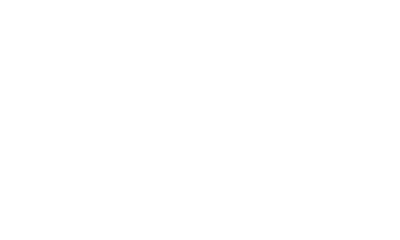
\includegraphics[width=\columnwidth]{images/exp1_scenes.png}
    \caption{Controlled-validation scenes.}
    \label{fig:exp1_scenes}
\end{figure}

Each scene is tested with the same basic procedure so that the differences in the results are caused by scene and ISAC configuration rather than changes in workflow.
The free-space and warehouse use cases use the sinusoidal trajectories of the robots shown in Figure \ref{fig:exp1_trajectories}.
The system is evaluated for $100$ time steps with a $0.2$ seconds interval, providing a $20$ seconds observation window.
At each step, propagation is computed and, when situation awareness is enabled, the sensing module produces detections that are filtered, clustered, tracked, and then used for sensing-informed beamforming.
The baseline does not use ISAC features and performs communication only, while the ISAC variants enable or disable specific functions such as MTI, tracking, beamwidth selection, and propagation depth in order to isolate one part of the proposed pipeline.

\begin{figure}[t]
    \centering
    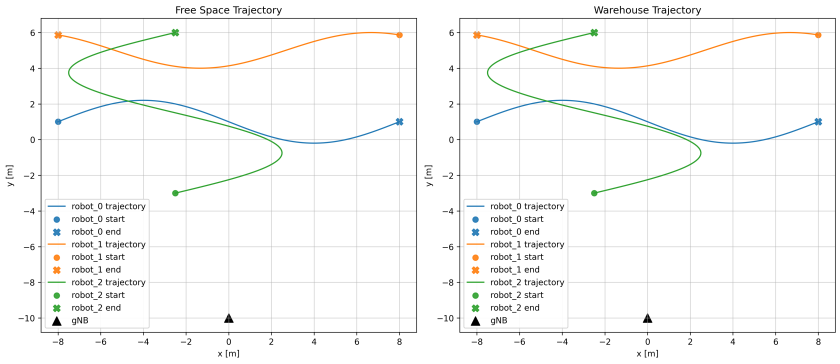
\includegraphics[width=\columnwidth]{images/exp1_trajectories.png}
    \caption{Deterministic robot trajectories used in the controlled
        validation scenes.}
    \label{fig:exp1_trajectories}
\end{figure}

The \texttt{isac\_full} variant test the whole pipeline.
The \texttt{isac\_no\_mti} variant disables only MTI to test whether removing static-reflection suppression affects detection stability.
The \texttt{isac\_narrow} and \texttt{isac\_wide} variants change only beamwidth to compare tighter target focusing against wider coverage under localization error.
The \texttt{isac\_deep} variant increases propagation depth to test whether additional multipath improves sensing or mainly adds clutter.
The \texttt{isac\_no\_tracker} variant disables temporal tracking to test whether raw frame-by-frame detections are sufficient for beamforming.
After each run, the estimated target positions are matched to the known ground truth from the trajectories with the Hungarian algorithm, where unmatched estimates are considered as false positives and unmatched targets are considered as missed detections.

\subsubsection{Free-Space Scene}
\label{subsubsec:controlled_validation_free_space}

The results in Table \ref{tab:exp1_fs_prop} shows that enabling ISAC reduces the mean path loss from $102.39$ dB to the range $84.39$--$86.82$dB.
The mean path delay remains at $54.10$ ns as the mean distance is same for all the variants.
The differences of performance is more observable in received power as in path loss.
Among the tested ablations, \texttt{isac\_wide} achieves the lowest path loss and the strongest received power, which indicates that the wider beam is beneficial when clutter is minimal.

\begin{table}[t]
    \centering
    \caption{Free-space propagation metrics.}
    \label{tab:exp1_fs_prop}
    \footnotesize
    \begin{tabular}{lccc}
        \hline
        Variant           & Path loss [dB] & Delay [ns] & Rx power [dBm] \\
        \hline
        baseline          & 102.39         & 54.10      & $-56.39$       \\
        isac\_full        & 86.30          & 54.10      & $-40.30$       \\
        isac\_no\_mti     & 85.53          & 54.10      & $-39.53$       \\
        isac\_narrow      & 86.82          & 54.10      & $-40.82$       \\
        isac\_wide        & 84.39          & 54.10      & $-38.39$       \\
        isac\_deep        & 85.54          & 54.10      & $-39.54$       \\
        isac\_no\_tracker & 85.43          & 54.10      & $-39.43$       \\
        \hline
    \end{tabular}
\end{table}

The sensing and tracking results in Table~\ref{tab:exp1_fs_sense} follow a similar trend.
The tracking-enabled ISAC variants achieve detection rates between $0.847$ and $0.903$, while their false-positive rates remain close to $0.018$--$0.019$.
Among them, \texttt{isac\_deep} achieves the highest detection rate $0.903$ and lowest missed-detection rate $0.097$, which shows that additional propagation depth can help to detect better but the gain over the other tracked variants is small.
However, the extra computation necessary for deeper propagation does not worth the gain.
The \texttt{isac\_no\_tracker} variant achieves the highest raw detection rate ($0.970$), but it also increases the false-positive rate to $0.176$.
This means that the tracker is useful because it trades raw sensitivity for cleaner detection.

\begin{table}[t]
    \centering
    \caption{Free-space sensing metrics.}
    \label{tab:exp1_fs_sense}
    \footnotesize
    \begin{tabular}{lccccc}
        \hline
        Variant           & Det.  & FPR   & Miss  & Err. [m] & Cont. \\
        \hline
        baseline          & 0.000 & 0.000 & 1.000 & --       & 0.000 \\
        isac\_full        & 0.847 & 0.019 & 0.153 & 1.148    & 0.550 \\
        isac\_no\_mti     & 0.897 & 0.018 & 0.103 & 1.125    & 0.537 \\
        isac\_narrow      & 0.897 & 0.018 & 0.103 & 1.125    & 0.537 \\
        isac\_wide        & 0.897 & 0.018 & 0.103 & 1.125    & 0.537 \\
        isac\_deep        & 0.903 & 0.018 & 0.097 & 1.126    & 0.510 \\
        isac\_no\_tracker & 0.970 & 0.176 & 0.030 & 1.208    & 0.583 \\
        \hline
    \end{tabular}
\end{table}

\subsubsection{Warehouse Scene}
\label{subsubsec:controlled_validation_warehouse}

In the warehouse scene, because of obstacles such racks and partial visibility create the clutter which makes sensing difficult.
The propagation results in Table \ref{tab:exp1_wh_prop} show that ISAC still improves communication, but the gain is smaller than free space case.
With ISAC, mean path loss drops from $109.16$ dB to $94.50$--$101.75$ dB across the ISAC variants.
Like in free space case, \texttt{isac\_wide} is the best in terms of path loss and received power, where it achieves $94.50$ dB path loss and $-48.50$ dBm received power.

\begin{table}[t]
    \centering
    \caption{Warehouse-scene propagation metrics.}
    \label{tab:exp1_wh_prop}
    \footnotesize
    \begin{tabular}{lccc}
        \hline
        Variant           & Path loss [dB] & Delay [ns] & Rx power [dBm] \\
        \hline
        baseline          & 109.16         & 53.95      & $-63.16$       \\
        isac\_full        & 97.90          & 53.95      & $-51.90$       \\
        isac\_no\_mti     & 97.39          & 53.95      & $-51.39$       \\
        isac\_narrow      & 101.75         & 53.95      & $-55.75$       \\
        isac\_wide        & 94.50          & 53.95      & $-48.50$       \\
        isac\_deep        & 97.44          & 53.95      & $-51.44$       \\
        isac\_no\_tracker & 98.52          & 53.95      & $-52.52$       \\
        \hline
    \end{tabular}
\end{table}

The sensing results in Table~\ref{tab:exp1_wh_sense} show that sensing in the warehouse scene is more difficult than in free space.
The tracked variants of ISAC detect only $0.280$--$0.290$ of the target instances and their missed-detection rates remain high around $0.710$--$0.720$.
This low detection rate is due to the racks, walls, and indoor objects block some target reflections.
As a result, some of true robot reflections are either too weak, too fragmented, or too close to clutter to survive the complete sensing pipeline and counted as missed detections.
The \texttt{isac\_deep} variant produce much higher false-positive rates, showing that deeper ray exploration adds more clutter and makes it harder to distinguish from the target reflections.
Like in free space, the tracking improve the detection rate and reduce the false-positive rate as the false-positive rate of \texttt{isac\_no\_tracker} is much higher than the others with tracking.

\begin{table}[t]
    \centering
    \caption{Warehouse-scene sensing metrics.}
    \label{tab:exp1_wh_sense}
    \footnotesize
    \begin{tabular}{lccccc}
        \hline
        Variant           & Det.  & FPR   & Miss  & Err. [m] & Cont. \\
        \hline
        baseline          & 0.000 & 0.000 & 1.000 & --       & 0.000 \\
        isac\_full        & 0.280 & 0.023 & 0.720 & 1.032    & 0.273 \\
        isac\_no\_mti     & 0.290 & 0.033 & 0.710 & 1.011    & 0.283 \\
        isac\_narrow      & 0.290 & 0.033 & 0.710 & 1.012    & 0.283 \\
        isac\_wide        & 0.290 & 0.022 & 0.710 & 1.012    & 0.283 \\
        isac\_deep        & 0.290 & 0.121 & 0.710 & 1.129    & 0.283 \\
        isac\_no\_tracker & 0.283 & 0.336 & 0.717 & 1.252    & 0.273 \\
        \hline
    \end{tabular}
\end{table}

This validation confirms two connected observations.
First, the framework behaves as expected in free space, where both communication and sensing benefit from favorable visibility.
Across both scenes, the wider beamwidth gives the best propagation result because it covers target positions uncertainty better than the narrower beam.
Increasing propagation depth improves detection rate slightly, but the gain is very small and, in the warehouse case, it increases false positive rate.
Second, the framework works in the warehouse case as well but the performance is degraded due to racks and partial visibility.
The no-tracker cases show that raw detections alone are not enough as it is needed to reduce the false-positive rate.

\subsection{Warehouse Use-Case Results}
\label{subsec:warehouse_usecase_results}

After the controlled validation, the framework proposed is applied to simulate the warehouse digital twin application.
The simulation running on NR baseline configuration without ISAC components and NR ISAC configuration are evaluated for 2x2, 4x4, and 8x8 gNB array sizes.
Both scenarios use the same warehouse layout, wireless node positions, robot mobility model, radio parameters, and application workload, so the comparison isolates the effect of enabling situation awareness in the Sionna-backed channel.

\subsubsection{Warehouse Digital Twin}

To evaluate the framework in a realistic 6G warehouse environment, we created a digital twin application for warehouse.
The whole workflow is managed by the a warehouse controller.
The controller communicates with package sensors, racks, temperature and humidity sensors, mobile robots, video clients, and cameras.
The package sensors and racks are stationary, while the robots move between the package sensor area, the racks and dropoff area.
The sensors report the status to the controller periodically.
According to the status of the sensors, the controller sends commands to the robots to pickup the packages, put them on the rack or drop off at the dropoff area.
The controller track the positions of the robots by communicating with the gNB which keeps the positions of the robots in the system state.
The robots are equipped with cameras on them for monitoring the packages, the racks, and the environment and the user can request the video stream from the cameras through the video clients.

Among the warehouse devices, the package sensors, rack sensors, temperature and humidity sensors are stationary while the robots are mobile.
The robots are main targets for the ISAC evaluation because they are mobile, the propagation conditions change frequently, and the robot positions are tracked by the gNB.
Other wireless devices create background traffic and competing wireless flows.
Therefore, this scenario tests whether ISAC can improve robot communication while keeping the rest of the warehouse workload active.

The performance is evaluated in terms of application-related KPIs, propagation-related KPIs, power consumption related KPIs and sensing related KPIs.
First, application flows are grouped by node type to measure throughput, delay, jitter, and packet loss.
Next, Sionna propagation traces are grouped by device type to explain the channel behavior.
Then, energy traces are used to measure the power consumption of gNB according to the array size and ISAC activation.
Finally, the ISAC detected-object output is used to evaluate robot detection, tracking continuity, and localization error.

\subsubsection{Application-related KPIs}

The application results in Fig.~\ref{fig:exp2_app} are considered first because
they show the end-to-end effect experienced by the warehouse traffic. At
$2\!\times\!2$, ISAC does not yet provide a stable system-level benefit:
controller throughput drops from $417.674$~kbps to $205.345$~kbps, and
package-sensor throughput drops from $22.990$~kbps to $6.634$~kbps. Robot
throughput increases slightly from $1159.444$~kbps to $1249.326$~kbps, but this
increase is accompanied by $15.439\%$ packet loss, so the small-array ISAC case
is better interpreted as unstable delivery rather than a useful gain.

\begin{figure}[t]
  \centering
  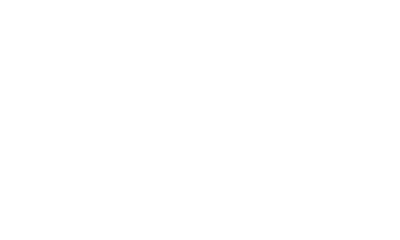
\includegraphics[width=\columnwidth]{images/exp2_app.png}
  \caption{Application-level KPIs under baseline and ISAC for the three gNB
    array sizes.}
  \label{fig:exp2_app}
\end{figure}

When the gNB array is increased to $4\!\times\!4$, the application behavior
changes because the ISAC configuration gains enough spatial resolution to
support the dominant mobile links. Controller and package-sensor throughput
return to the baseline range, while robot throughput increases to
$1582.081$~kbps compared with the baseline value of $1328.452$~kbps. The
$8\!\times\!8$ ISAC case keeps the same robot-dominant trend but reduces robot
throughput to $1445.378$~kbps, so the larger array does not provide a
proportional additional application gain. The application layer therefore
identifies $4\!\times\!4$ as the first array size where ISAC becomes useful for
the warehouse workload.

\subsubsection{Propagation-related KPIs}

The propagation results in Fig.~\ref{fig:exp2_prop} explain why the
application-level gain appears only after the array reaches $4\!\times\!4$.
For robot links, baseline path loss decreases from $83.948$~dB at
$2\!\times\!2$ to approximately $69.2$~dB at $4\!\times\!4$ and
$8\!\times\!8$. Under ISAC, the same trend is stronger: robot path loss falls
from $82.318$~dB at $2\!\times\!2$ to $57.359$~dB at $4\!\times\!4$ and then
remains almost unchanged at $8\!\times\!8$. This channel-level saturation
matches the application-level saturation, because most of the useful ISAC gain
is already obtained at $4\!\times\!4$.

\begin{figure}[t]
  \centering
  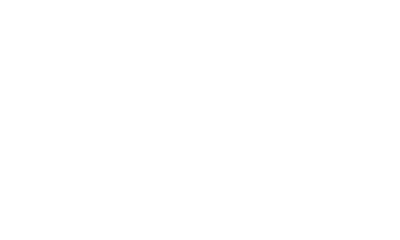
\includegraphics[width=\columnwidth]{images/exp2_prop.png}
  \caption{Propagation KPIs grouped by wireless node category, with solid bars
    for Native and hatched bars for Sionna Pattern.}
  \label{fig:exp2_prop}
\end{figure}

The propagation improvement is not uniform across all warehouse devices, and
this selectivity is important for interpreting the system result. Rack-sensor
links also benefit from ISAC, with roughly $20$~dB lower path loss than the
baseline across the tested array sizes. In contrast, package, temperature, and
humidity sensors experience higher path loss under ISAC than under the
baseline. The overall throughput improvement is therefore driven mainly by the
mobile robot links, which are the links most directly aligned with the
sensing-informed beamforming objective.

\subsubsection{Power Consumption related KPIs}

The power results in Fig.~\ref{fig:exp2_power} are evaluated after the
communication and propagation results because they determine whether the
observed gains are practically affordable. The dominant power factor is the gNB
array size rather than ISAC activation alone. The gNB average power rises from
approximately $25.6$~W at $2\!\times\!2$ to $51.3$~W at $4\!\times\!4$, and
then to about $145$~W at $8\!\times\!8$. The corresponding gNB energy increases
from about $3.1$~kJ to $6.15$~kJ and then to approximately $17.4$~kJ.

\begin{figure}[t]
  \centering
  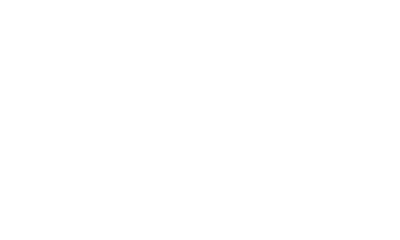
\includegraphics[width=\columnwidth]{images/exp2_power.png}
  \caption{Average power and consumed energy under baseline and ISAC.}
  \label{fig:exp2_power}
\end{figure}

This energy trend changes the interpretation of the larger array sizes. At the
system level, total reported energy is nearly identical between baseline and
ISAC for the $4\!\times\!4$ and $8\!\times\!8$ cases, while ISAC slightly
improves the useful throughput. However, the $8\!\times\!8$ array requires much
higher gNB power without giving a proportional communication gain over
$4\!\times\!4$. Therefore, the energy results reinforce the application and
propagation results: $4\!\times\!4$ is the balanced operating point for the
tested warehouse workload.

\subsubsection{Sensing and Localization}

The sensing results are evaluated last because they are available only in the
ISAC scenario and because they explain whether the communication gains are
supported by meaningful target awareness. Fig.~\ref{fig:exp2_sense} shows that
the main sensing improvement occurs when the gNB array is increased from
$2\!\times\!2$ to $4\!\times\!4$. The detection rate rises from $0.485$ to
$0.523$, and the missed-detection rate correspondingly falls from $0.515$ to
approximately $0.477$. The $8\!\times\!8$ case changes these values only
slightly, with a detection rate of $0.526$, so sensing also saturates after the
$4\!\times\!4$ configuration.

\begin{figure}[t]
  \centering
  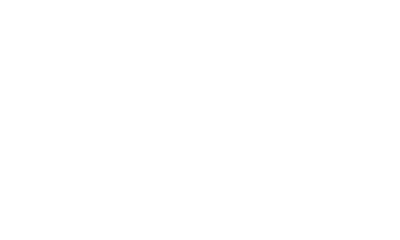
\includegraphics[width=\columnwidth]{images/exp2_sense.png}
  \caption{Sensing KPIs for the ISAC warehouse scenario.}
  \label{fig:exp2_sense}
\end{figure}

False positives and track continuity clarify the quality of those detections.
Validated false positives are already low at $2\!\times\!2$ and fall to zero
for both $4\!\times\!4$ and $8\!\times\!8$. Track continuity remains close to
unity across the three array sizes, which means that once a valid robot
detection sequence is formed, the exported identity remains stable. The larger
arrays therefore improve sensing mostly by increasing valid detection
opportunities and reducing unstable detections, not by fundamentally changing
the tracking behavior.

\begin{figure}[t]
  \centering
  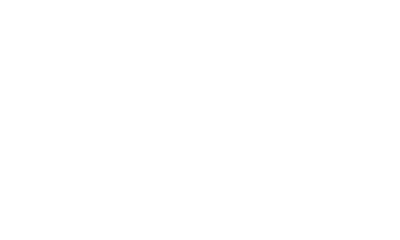
\includegraphics[width=\columnwidth]{images/exp2_loc_err.png}
  \caption{Localization-error distribution for the ISAC warehouse scenario.}
  \label{fig:exp2_loc_err}
\end{figure}

The localization-error distribution in Fig.~\ref{fig:exp2_loc_err} shows the
same stability effect from a different angle. The $2\!\times\!2$ configuration
has the lowest median error at $0.384$~m, but it also has the largest maximum
error at $10.427$~m. The $4\!\times\!4$ and $8\!\times\!8$ configurations have
slightly higher median errors of about $0.577$~m, but their maximum errors are
reduced to around $4.5$~m and their upper-tail errors are lower. Thus, the
larger arrays do not mainly improve pointwise median localization; instead,
they suppress large-error outliers and make the sensing output more stable.

Overall, the warehouse use-case experiment shows that ISAC benefit depends on
sufficient antenna-array support. The $2\!\times\!2$ ISAC configuration is not
stable enough for the mixed warehouse workload, whereas the $4\!\times\!4$
configuration improves the dominant robot communication links, improves sensing
stability, and avoids the much higher gNB power cost of $8\!\times\!8$. The
results therefore support $4\!\times\!4$ as the most balanced configuration
among the tested cases.


\section{Conclusion and Future Work}
\label{sec:conclusion}

This paper presented a situation-aware ISAC co-simulation framework for 6G
smart warehouses. The framework connects Sionna RT with ns-3/5G~LENA so that
site-specific ray tracing, sensing, tracking, adaptive beamforming, and NR
communication can be evaluated in one workflow. The sensing module converts
ray-traced reflections into target detections, the tracking module stabilizes
those detections over time, and the beamforming module uses the confirmed
target positions to update the communication link.

The controlled validation shows that the framework behaves as expected when
the scene becomes more difficult. In free space, visibility is favorable, so
ISAC reduces the mean path loss by up to about $18$~dB and keeps the
false-positive rate low when tracking is enabled. In the warehouse scene, ISAC
still improves propagation, with the widest tested beam giving the strongest
path-loss reduction. However, racks, walls, and partial visibility reduce the
detection rate and increase missed detections. This means that the main
warehouse sensing problem is not pointwise localization accuracy after a target
is detected, but maintaining complete and continuous detections in clutter. The
ablation results also show two important trade-offs: deeper propagation gives
only a small detection gain and can add false positives, while removing the
tracker increases raw detections but makes the output much less clean.

The end-to-end warehouse Digital Twin confirms that these controlled findings
matter at application level. The $2{\times}2$ gNB array is not sufficient for a
stable ISAC gain because robot traffic becomes less reliable. The $4{\times}4$
array gives the best operating point: it improves robot-link propagation and
throughput, keeps the rest of the warehouse traffic usable, improves sensing
stability, and avoids the large power increase of the $8{\times}8$ array. The
$8{\times}8$ case provides more antenna resources, but its extra energy cost is
not matched by a proportional communication or sensing improvement.

These results show that ISAC should not be evaluated from sensing accuracy or
communication throughput alone. A useful warehouse deployment must balance all
three dimensions: reliable target awareness, useful link improvement, and
reasonable energy cost. Future work should therefore focus on more robust
clutter handling, stronger track continuity in dense indoor scenes, and
beam-management methods that combine target position with channel state
information. The evaluation should also be extended with more traffic loads,
random seeds, robot routes, and warehouse layouts so that the operating limits
of the framework can be characterized more completely.


\begin{thebibliography}{99}

\bibitem{ref:positioning_6g}
H.~Wymeersch \emph{et~al.}, ``Positioning and sensing in 6G: Gaps,
challenges, and opportunities,'' \emph{IEEE Vehicular Technology Magazine},
2022. % TODO: complete citation

\bibitem{ref:multimodal_bf}
Y.~Heng \emph{et~al.}, ``AI-enabled multimodal beamforming for next-generation
wireless systems: A survey,'' \emph{IEEE Communications Surveys \& Tutorials},
2023. % TODO: complete citation

\bibitem{ref:predictive_handover}
Authors, ``Memory-full context-aware predictive mobility management in
dual-connectivity 5G networks,'' \emph{IEEE Trans.\ on Mobile Computing}.
% TODO: complete citation

\bibitem{ref:sionna_rt}
J.~Hoydis \emph{et~al.}, ``Sionna RT: Differentiable ray tracing for radio
propagation modeling,'' NVIDIA, 2023.
\url{https://nvlabs.github.io/sionna/}. % TODO: confirm citation

\bibitem{ref:ns3sionna}
A.~Authors, ``Ns3Sionna: Integrating Sionna RT GPU-accelerated ray tracing
into ns-3,'' in \emph{Proc.\ Workshop on ns-3 (WNS3)}, 2024.
% TODO: complete citation

\bibitem{ref:5glena}
N.~Patriciello \emph{et~al.}, ``An E2E simulator for 5G NR networks,''
\emph{Simulation Modelling Practice and Theory}, vol.~96, 2019.
% TODO: confirm citation

\bibitem{ref:tr38901}
3GPP, ``Study on channel model for frequencies from 0.5 to 100 GHz,''
TR~38.901, 3rd Generation Partnership Project. % TODO: version/date

\bibitem{ref:dbscan}
M.~Ester, H.-P.~Kriegel, J.~Sander, and X.~Xu, ``A density-based algorithm
for discovering clusters in large spatial databases with noise,'' in
\emph{Proc.\ KDD}, 1996, pp.~226--231.

\bibitem{ref:hungarian}
H.~W.~Kuhn, ``The Hungarian method for the assignment problem,''
\emph{Naval Research Logistics Quarterly}, vol.~2, no.~1--2,
pp.~83--97, 1955.

\bibitem{ref:simu5g}
G.~Nardini \emph{et~al.}, ``Simu5G---an OMNeT++ library for end-to-end
performance evaluation of 5G networks,'' \emph{IEEE Access},
vol.~8, 2020. % TODO: confirm citation

\end{thebibliography}


\begin{IEEEbiography}[{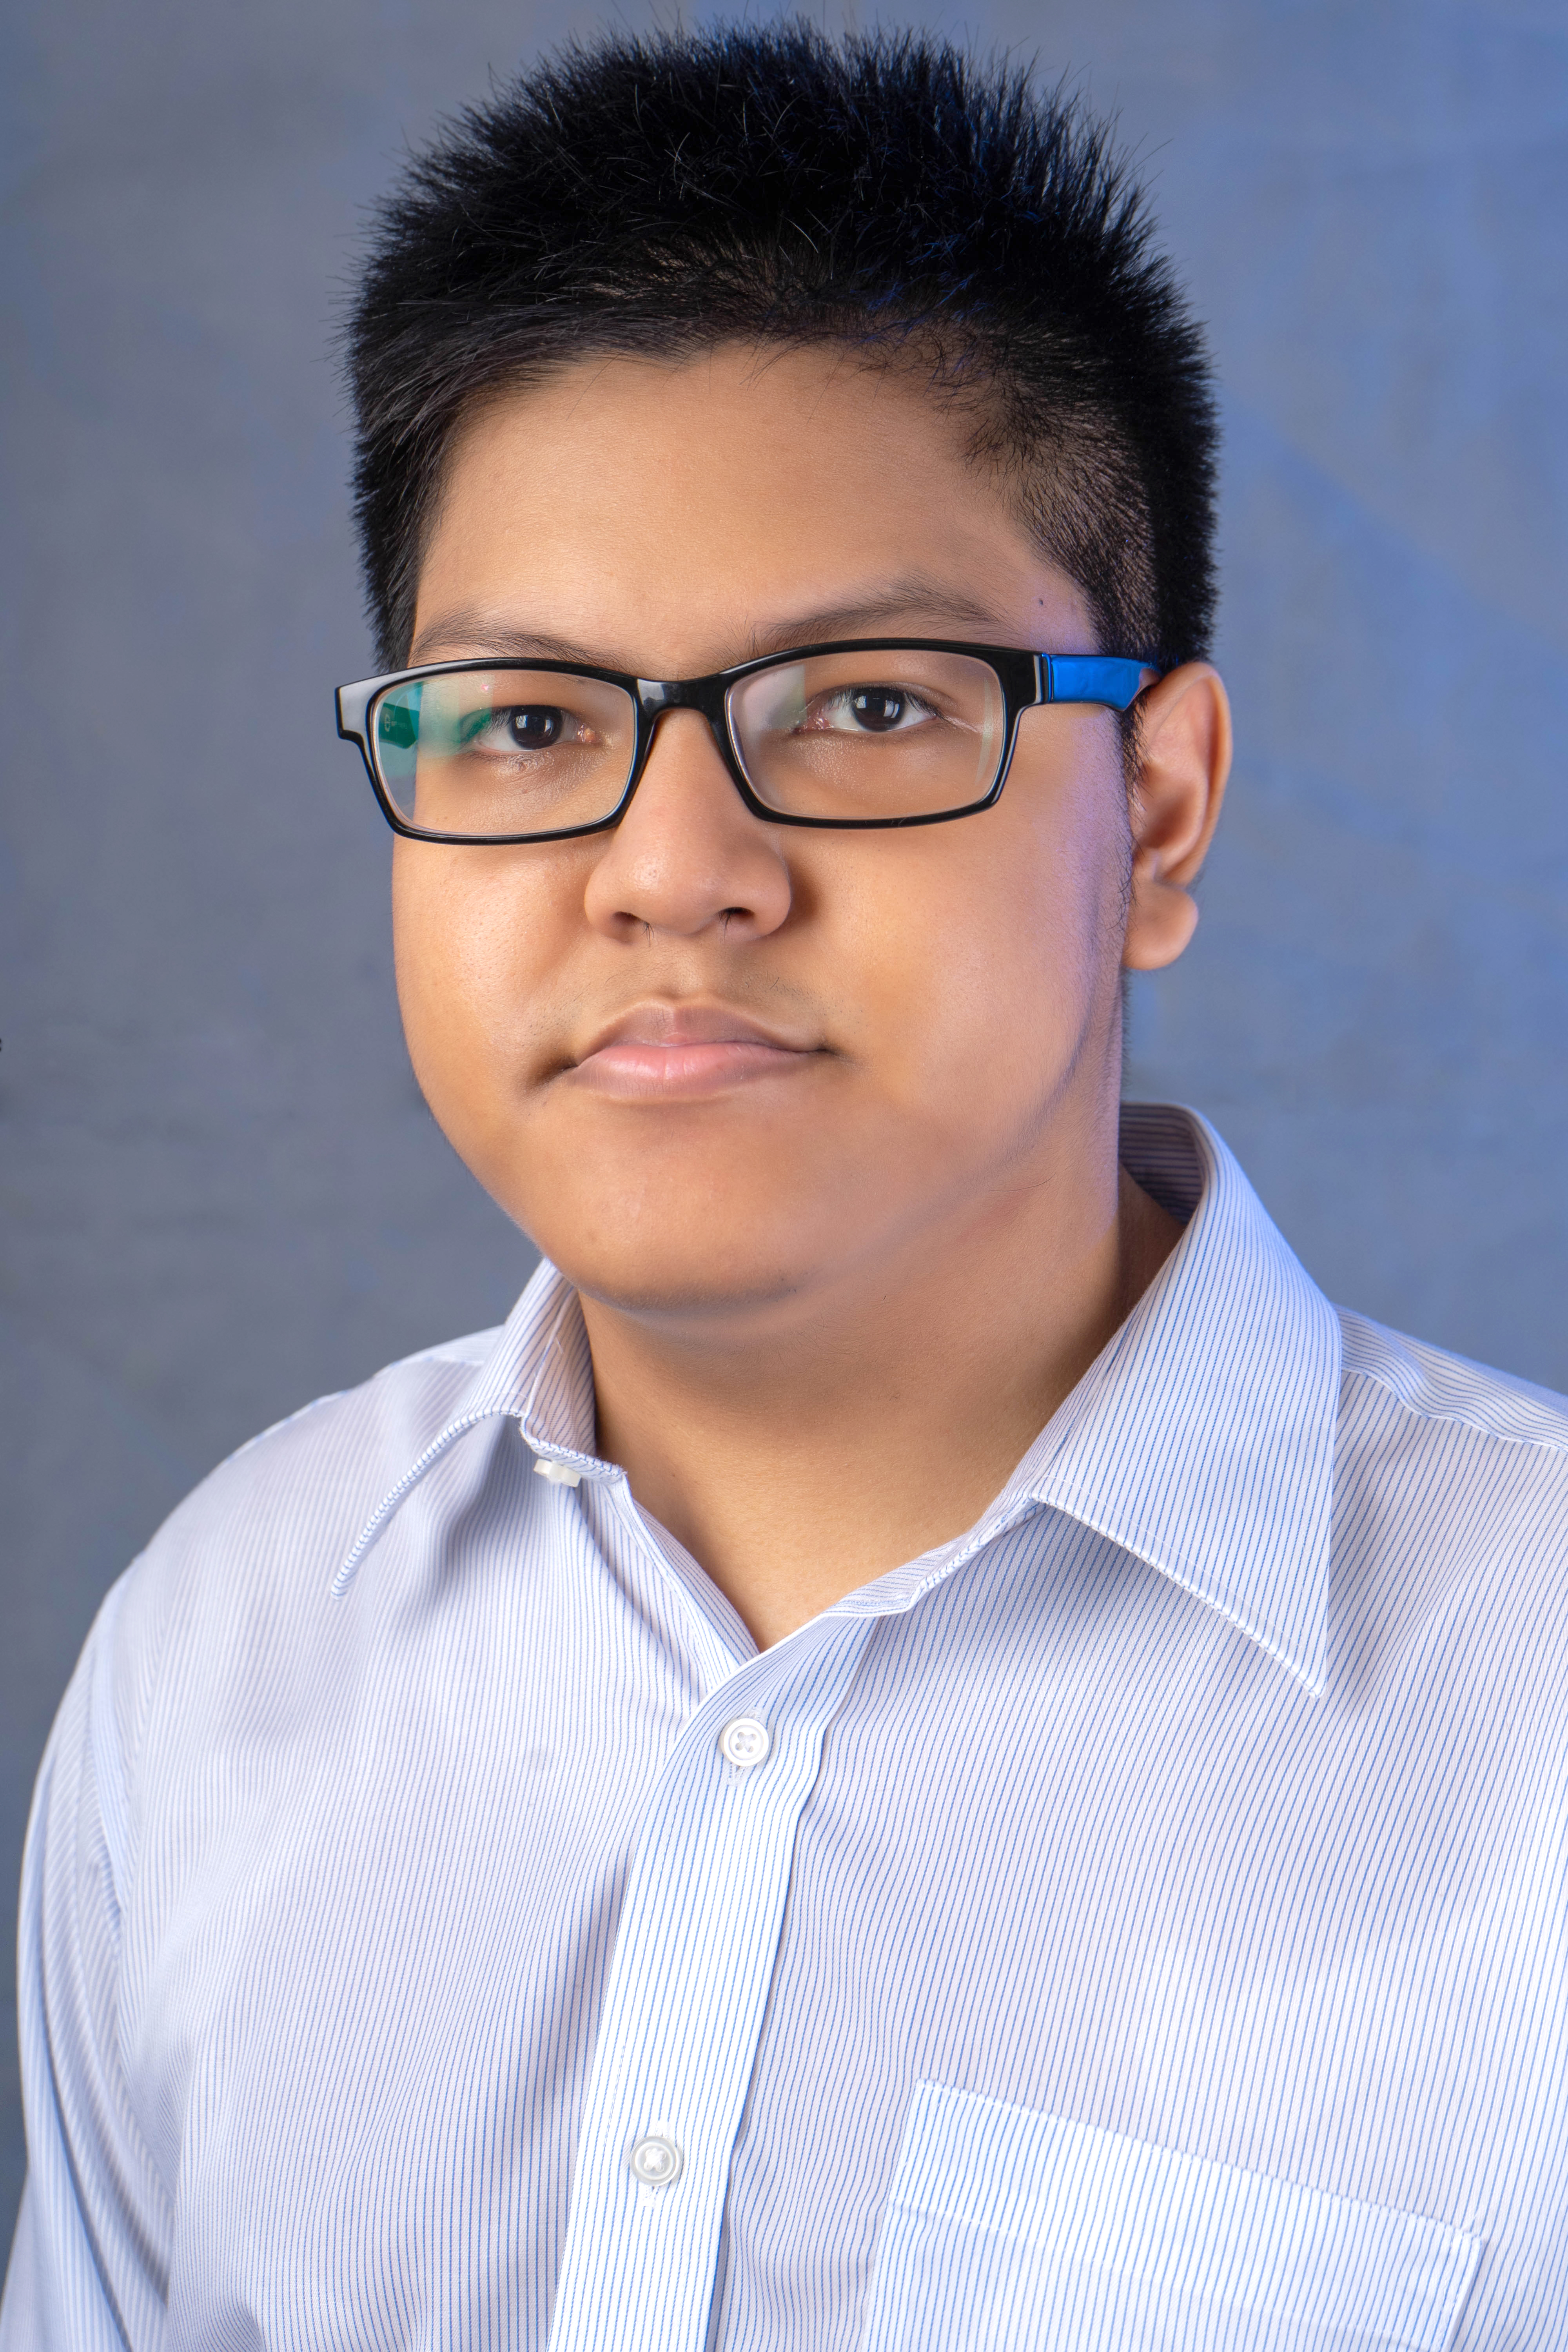
\includegraphics[width=1in,height=1.25in,clip,keepaspectratio]{images/Aung_Kaung_MYAT.jpg}}]{Aung Kaung MYAT}
is a PhD researcher at SAMOVAR, T\'el\'ecom SudParis, Institut Polytechnique
de Paris. His research interests include 6G access networks, integrated
sensing and communication, ray-tracing-based channel modelling, and
Digital-Twin-driven network simulation.
\end{IEEEbiography}

\begin{IEEEbiographynophoto}{Hrishikesh Dutta}
is with SAMOVAR, T\'el\'ecom SudParis, Institut Polytechnique de Paris.
His research interests include wireless networks, machine learning for
communications, and next-generation system design.
\end{IEEEbiographynophoto}

\begin{IEEEbiographynophoto}{Roberto Minerva}
is with SAMOVAR, T\'el\'ecom SudParis, Institut Polytechnique de Paris.
His research interests include Internet of Things, edge computing, and
service architectures for next-generation networks.
\end{IEEEbiographynophoto}

\begin{IEEEbiographynophoto}{Noel Crespi}
is a Professor at SAMOVAR, T\'el\'ecom SudParis, Institut Polytechnique de
Paris. His research interests cover service engineering, future networks,
and the convergence of telecommunications and information services.
\end{IEEEbiographynophoto}


\end{document}


